\chapter{Basic concepts} \label{ch:intro}

\section{\mlab in the School of Engineering, University of Edinburgh}
\mlab is currently available under Microsoft Windows and Linux operating systems in the School of Engineering Computing Labs, and also under Microsoft Windows in all of the University's Open Access Computing Labs\footnote{(\href{http://www.ed.ac.uk/information-services/computing/desktop-personal/open-access/locations}{http://www.ed.ac.uk/information-services/computing/desktop-personal/open-access/locations})}. \mlab is available to both students and staff of the University under a site license. More information on how to \href{http://www.ed.ac.uk/information-services/computing/desktop-personal/software/main-software-deals/matlab}{get access to \mlab} on your computer can be found at the Univeristy's Information Services website\footnote{(\href{http://www.ed.ac.uk/information-services/computing/desktop-personal/software/main-software-deals/matlab}{http://www.ed.ac.uk/information-services/computing/desktop-personal/software/main-software-deals/matlab})}

\section{The \mlab environment}
When you launch \mlab you are presented with the \mlab desktop (Figure~\ref{fig:matlab_desktop}) which, by default, is divided into 4 windows:
\begin{enumerate}
\item Command Window: This is the main window, and contains the command prompt (\texttt{>>}). This is where you will type all commands.
\item Command History: Displays a list of previously typed commands. The command history persists across multiple sessions and commands can be dragged into the Command Window and edited, or double-clicked to run them again.
\item Workspace: Lists all the variables you have generated in the current session. It shows the type and size of variables, and can be used to quickly plot, or inspect the values of variables.
\item Current Directory: Shows the files and folders in the current directory. The path to the current directory is listed near the top of the \mlab desktop. By default, a \mlab folder is created in your home directory, and this is where you should save your work.
\end{enumerate}
You will use and become more familiar with the different areas of the \mlab desktop as you progress through this course. \\
\begin{figure}
	\myfloatalign
	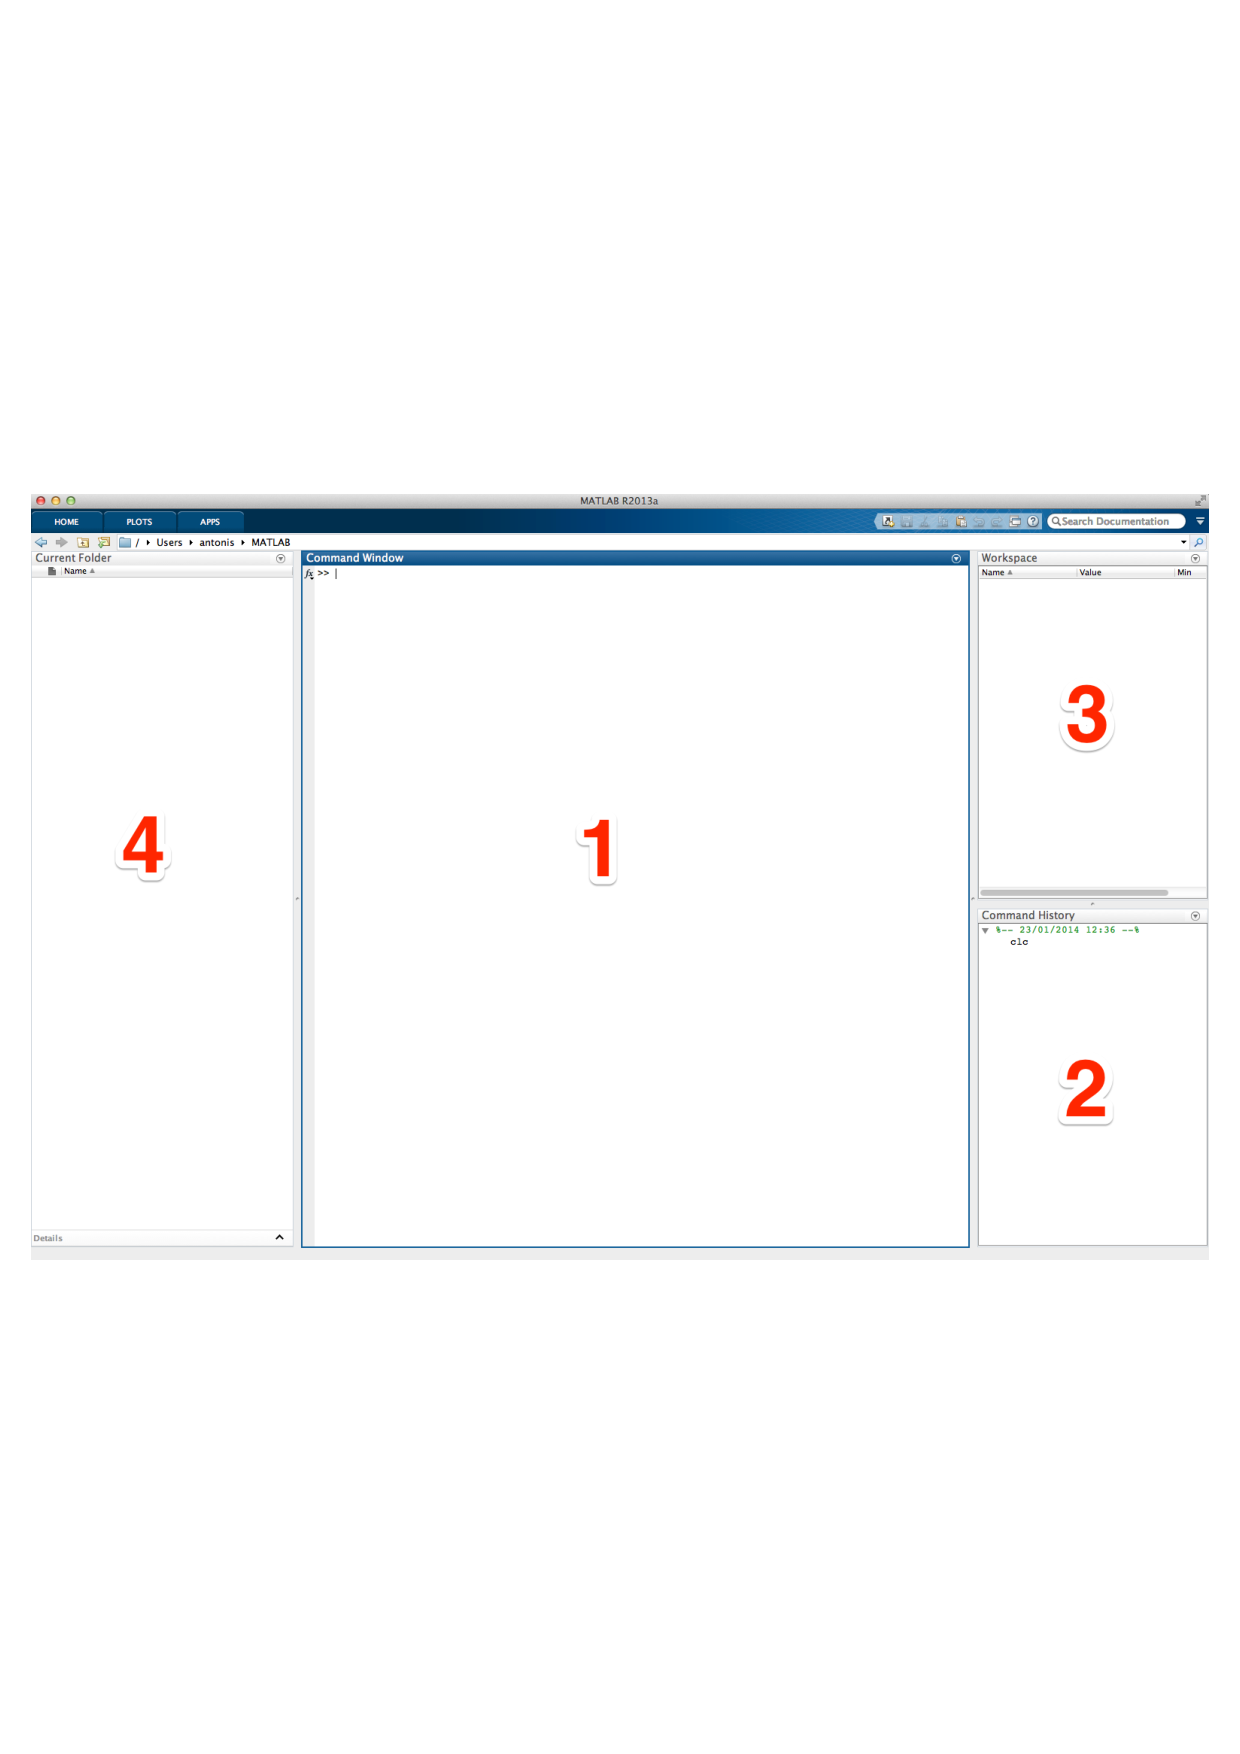
\includegraphics[width=\linewidth]{Graphics/Unit01/matlab_desktop}
	\caption{The \mlab desktop}
	\label{fig:matlab_desktop}
\end{figure}

%%%%%%%%%%%%%%%%%%%%%%%%%%%%%%%%%%%%%%%%%%%%%%
% Screencast: The MATLAB desktop
%%%%%%%%%%%%%%%%%%%%%%%%%%%%%%%%%%%%%%%%%%%%%%
\addtolength{\parindent}{-4mm}
\fcolorbox{myborderblue}{myblue}{%
\begin{minipage}{\linewidth}
\begin{minipage}{6mm}

\includegraphics[scale=0.03]{Graphics/General/screencast_icon}
\end{minipage}
\href{https://youtu.be/PfklSSxZSZU}{\screencast{The \mlab desktop}}\\
(https://youtu.be/PfklSSxZSZU)
\end{minipage}%
}\\
\addtolength{\parindent}{4mm}
\graffito{Remember you can pause the screencasts at any time and try the examples for yourself.}

\section{Basic calculations}
\mlab can perform basic calculations such as those you are used to doing on your calculator. Listings~\ref{lst:add}--\ref{lst:trig2} gives some simple examples (and results) of arithmetic operations, exponentials and logarithms, trigonometric functions, and complex numbers that can be entered in the Command Window.
\begin{lstlisting}[caption={Addition},label=lst:add]
>> 4+3
ans = 
	 7
\end{lstlisting}	 

\graffito{Try using \mlab as an expensive calculator!} 
\begin{lstlisting}[caption={Exponentiation},label=lst:exp]
>> 2^2
ans = 
	 4
\end{lstlisting}	

\begin{lstlisting}[caption={Trigonometry},label=lst:trig1]
>> sin(2*pi)+exp(-3/2)
ans = 
	 0.2231
\end{lstlisting}
\graffito{The arguments to trigonometric functions should be given in radians.}
\subsubsection{Comments:}
\begin{itemize}
\item \mlab has pre-defined constants \eg\ $\pi$ may be typed as \mcode{pi}.
\item You must explicitly type all arithmetic operations \eg\ \mcode{sin(2*pi)} not \mcode{sin(2pi)}.
\item \mcode{sin(x)} and \mcode{exp(x)} correspond to $\sin(x)$ and $e^x$ respectively.
\end{itemize}

\begin{lstlisting}[caption={Complex numbers},label=lst:complex]
>> 5+5j
ans =
	 5.0000 + 5.0000i
\end{lstlisting}

\subsubsection{Comments:}
\begin{itemize}
\item Complex numbers can be entered using the basic imaginary unit \mcode{i} or \mcode{j}.
\end{itemize}

\begin{lstlisting}[caption={More trigonometry},label=lst:trig2]	 
>> atan(5/5)
ans =
	 0.7854
	 
>> 10*log10(0.5)
ans =
	 -3.0103
\end{lstlisting}

\subsubsection{Comments:}
\begin{itemize}
\item \mcode{atan(x)} and \mcode{log10(x)} correspond to $\tan^{-1}(x)$ and $log_{10}(x)$ respectively.
\end{itemize}

\begin{table}[h]
	\caption{Arithmetic operations}
	\label{tab:arith_ops}
	\myfloatalign
	\begin{tabular}{ll}\toprule
	\spacedlowsmallcaps{Command} & \spacedlowsmallcaps{Description}\\ \midrule
	\mcode{+} & Addition \\
	\mcode{-} & Subtraction \\
	\mcode{*} & Multiplication \\
	\mcode{/} & Division \\
	\mcode{^} & Exponentiation \\
	\bottomrule
	\end{tabular}
\end{table}

\addtolength{\parindent}{-4mm}
\fcolorbox{myborderblue}{myblue}{%
\begin{minipage}{\linewidth}
\begin{minipage}{6mm}

\includegraphics[scale=0.03]{Graphics/General/help_icon}
\end{minipage}
\textit{Built-in functions} \\
There are many other built-in \mlab functions for performing basic calculations. These can be searched from the Help Browser which is opened by clicking on its icon (like the icon used to indicate this Hints and Tips section) in the \mlab desktop toolbar.
\end{minipage}%
}\\
\addtolength{\parindent}{4mm}

%%%%%%%%%%%%%%%%%%%%%%%%%%%%%%%%%%%%%%%%%%%%%%
% Exercise 1: Basic calculations
%%%%%%%%%%%%%%%%%%%%%%%%%%%%%%%%%%%%%%%%%%%%%%
\addtolength{\parindent}{-4mm}
\fcolorbox{myborderblue}{myblue}{%
\begin{minipage}{\linewidth}
\begin{minipage}{6mm}

\includegraphics[scale=0.035]{Graphics/General/exercise_icon}
\end{minipage}
\exercise{\textit{Exercise 1: Basic calculations}}
\begin{enumerate}
\item Launch \mlab and explore the different areas of the \mlab desktop.
\item Try the basic calculations given in Listings~\ref{lst:add}--\ref{lst:trig2}, and check you get the correct answers.
\item \textit{Arithmetic operations} \\
Compute the following:
	\begin{itemize}
	\item $\frac{2^5}{2^5-1}$ and compare with $\left( 1-\frac{1}{2^5} \right) ^ {-1}$
	\item $\frac{\sqrt{5}-1}{(\sqrt{5}+1)^2}$
	\end{itemize}
\footnotesize{\textit{[Answers: 1.0323, 1.0323, 0.1180]}}
\normalsize
\item \textit{Exponentials and logarithms} \\
Compute the following:
	\begin{itemize}
	\item $e^3$
	\item $ln(e^3)$
	\item $log_{10}(e^3)$
	\item $log_{10}(10^5)$
	\end{itemize}
\footnotesize{\textit{[Answers: 20.0855, 3, 1.3029, 5]}}
\normalsize
\item \textit{Trigonometric operations} \\
Compute the following:
	\begin{itemize}
	\item $\sin(\frac{\pi}{6})$
	\item $\cos(\pi)$
	\item $\tan(\frac{\pi}{2})$
	\item $\sin^2(\frac{\pi}{6}) + \cos^2(\frac{\pi}{6})$
	\end{itemize}
\footnotesize{\textit{[Answers: 0.5, -1, 1.6331E16, 1]}}
\normalsize
\end{enumerate}
%%%%%%%%%%%%%%%%%%%%%%%%%%%%%%%%%%%%%%%%%%%%%%
% Screencast: Exercise 1 Solutions
%%%%%%%%%%%%%%%%%%%%%%%%%%%%%%%%%%%%%%%%%%%%%%
\begin{minipage}{6mm}

\includegraphics[scale=0.03]{Graphics/General/screencast_icon}
\end{minipage}
\href{https://youtu.be/rZuAns0iEt4}{\screencast{Exercise 1 Solutions}}\\
(https://youtu.be/rZuAns0iEt4)
%\href{http://www.eng.ed.ac.uk/teaching/courses/matlab/unit01/Ex1-Solutions.shtml}{\screencast{Exercise 1 Solutions}}\\
%(http://www.eng.ed.ac.uk/teaching/courses/matlab/unit01/Ex1-Solutions.shtml)
\end{minipage}%
}\\
\addtolength{\parindent}{4mm}

You may have noticed that the result of each of the basic calculations you performed was always assigned to a variable called \mcode{ans}. Variables are a very important concept in \mlab.

\section{Variables and arrays}
A variable is a symbolic name associated with a value. The current value of the variable is the data actually stored in the variable. Variables are very important in \mlab because they allow us to easily reference complex and changing data. Variables can reference different data types \ie\ scalars, vectors, arrays, matrices, strings \etc. Variable names must consist of a letter which can be followed by any number of letters, digits, or underscores. \mlab is case sensitive \ie\ it distinguishes between uppercase and lowercase letters \eg\ \mcode{A} and \mcode{a} are not the same variable.

Variables you have created in the current \mlab session can be viewed in a couple of different ways. The Workspace (shown in Figure~\ref{fig:matlab_desktop}) lists all the current variables and allows you to easily inspect their type and size, as well as quickly plot them. Alternatively, the \mcode{whos} command can be typed in the Command Window and provides information about the type and size of current variables. Listing~\ref{lst:whos} shows the output of the \mcode{whos} command after storing and manipulating a few variables.

\begin{lstlisting}[caption={Using the \mcode{whos} command},label=lst:whos]
>> a = 2
a = 
	 2
>> b = 3
b = 
	 3
>> c = a*b
c = 
	 6
>> edinburgh = a+5
edinburgh = 
	 7
>> whos
  Name           Size            Bytes  Class     Attributes

  a              1x1                 8  double              
  b              1x1                 8  double              
  c              1x1                 8  double              
  edinburgh      1x1                 8  double
\end{lstlisting}

Arrays are lists of numbers or expressions arranged in horizontal rows and vertical columns. A single row, or single column array is called a vector. An array with $m$ rows and $n$ columns is called a matrix of size $m \times n$. Listings~\ref{lst:row_vect}--\ref{lst:ranges} demonstrate how to create row and column vectors, and matrices in \mlab.

\begin{lstlisting}[caption={Creating a row vector},label=lst:row_vect]
>> x = [1 2 3]
x = 
	 1    2    3
\end{lstlisting}
\begin{itemize}
\item Square brackets are used to denote a vector or matrix.
\item Spaces are used to denote columns.
\end{itemize}

\begin{lstlisting}[caption={Creating a column vector},label=lst:col_vect]	
>> y = [4; 5; 6]
y = 
	 4
	 5
	 6
\end{lstlisting}
\begin{itemize}
\item The semicolon operator is used to separate columns.
\end{itemize}

\begin{lstlisting}[caption={The transpose operator},label=lst:transpose]	
>> x'
ans = 
	  1
	  2
	  3
	 
>> y'
ans =
	  4    5    6
\end{lstlisting}
\begin{itemize}
\item The single quotation mark \mcode{'} transposes arrays, i.e. the rows and columns are interchanged so that the first column becomes the first row etc...
\end{itemize}

A more efficient method for entering vectors, especially those that contain many values, is to use ranges. Instead of entering each individual value separately, a range of values can be defined as shown in Listing~\ref{lst:ranges}.
\newpage
\begin{lstlisting}[caption={Creating vectors using ranges},label=lst:ranges]	
>> z = 8:1:10
z = 
	 8    9    10
	 
>> v = linspace(0,10,5)
v =
	 0    2.5000    5.0000    7.5000    10.0000
\end{lstlisting}

\subsubsection{Comments:}
\begin{itemize}
\item A range can be created using the colon operator, \eg\ \mcode{8:1:10} means create a range that starts at 8 and goes up in steps of size 1 until 10.
\item A range can also be created using the \mcode{linspace} function, \\ \eg\ \mcode{linspace(0,10,5)} means create a range between 0 and 10 with 5 linearly spaced elements.
\end{itemize}

\addtolength{\parindent}{-4mm}
\fcolorbox{myborderblue}{myblue}{%
\begin{minipage}{\linewidth}
\begin{minipage}{6mm}

\includegraphics[scale=0.03]{Graphics/General/help_icon}
\end{minipage}
\mcode{clear} \textit{and} \mcode{clc} \textit{commands} \\
The \mcode{clear} command can be used if you want to clear the current workspace of all variables. Additionally, the \mcode{clc} command can be used to clear the Command Window, i.e. remove all text.
\end{minipage}%
}\\
\addtolength{\parindent}{4mm}
\vspace{5mm}

%%%%%%%%%%%%%%%%%%%%%%%%%%%%%%%%%%%%%%%%%%%%%%
% Screencast: Variables and simple arrays
%%%%%%%%%%%%%%%%%%%%%%%%%%%%%%%%%%%%%%%%%%%%%%
\addtolength{\parindent}{-4mm}
\fcolorbox{myborderblue}{myblue}{%
\begin{minipage}{\linewidth}
\begin{minipage}{6mm}

\includegraphics[scale=0.03]{Graphics/General/screencast_icon}
\end{minipage}
\href{https://youtu.be/Nsme7btg75U}{\screencast{Variables and simple arrays}}\\
(https://youtu.be/Nsme7btg75U)
%\href{http://www.eng.ed.ac.uk/teaching/courses/matlab/unit01/variables-arrays.shtml}{\screencast{Variables and simple arrays}}\\
%(http://www.eng.ed.ac.uk/teaching/courses/matlab/unit01/variables-arrays.shtml)
\end{minipage}%
}\\
\addtolength{\parindent}{4mm}

\mlab excels at matrix operations, and consequently the arithmetic operators such as multiplication (\mcode{*}), division (\mcode{/}), and exponentiation (\mcode{^}) perform matrix multiplication, division, and exponentiation, when used on a vector, by default. To perform an element-by-element multiplication, division, or exponentiation you must precede the operator with a dot. Table~\ref{tab:arith_ops_elemental} and Listing~\ref{lst:dot} demonstrate the dot operator.

\begin{lstlisting}[caption={The dot operator},label=lst:dot]
>> clear
>> a = [2 3; 5 1]
a = 
	 2    3
	 5    1
>> b = [4 7; 9 6]
b = 
	 4    7
	 9    6
>> a*b
ans = 
	35	 32
	29	 41
>> a.*b
ans = 
	 8    21
	45	  6
>> c = [1 2 3 4]
c = 
	 1    2    3    4
>> a*c
??? Error using ==> mtimes
Inner matrix dimensions must agree.
>> a.*c
??? Error using ==> mtimes
Matrix dimensions must agree.
\end{lstlisting}

\subsubsection{Comments:}
\begin{itemize}
\item The dot operator signifies an element-by-element operation. The dot can be used for multiplication \mcode{.*}, division \mcode{./}, or exponentiation \mcode{.^} of elements of vectors that are the same size. Omitting the dot before an arithmetic operator means \mlab performs the matrix version of the operation.
\item On Line 21 we tried to perform a matrix multiplication of a 2$\times$2 matrix with a 1$\times$4 matrix. This results in an error because you can only multiply two matrices if the number of columns in the first equals the number of rows in the second.
\item On Line 24 we get a similar error if we try to perform an element-by-element multiplication, as this does not make any sense for matrices of different sizes.
\end{itemize}

\begin{table}[h]
	\caption{Element-by-element arithmetic operations}
	\label{tab:arith_ops_elemental}
	\myfloatalign
	\begin{tabular}{ll}\toprule
	\spacedlowsmallcaps{Command} & \spacedlowsmallcaps{Description}\\ \midrule
	\mcode{.*} & Element-by-element multiplication \\
	\mcode{./} & Element-by-element division \\
	\mcode{.^} & Element-by-element exponentiation \\
	\bottomrule
	\end{tabular}
\end{table}

%%%%%%%%%%%%%%%%%%%%%%%%%%%%%%%%%%%%%%%%%%%%%%
% Screencast: The dot operator
%%%%%%%%%%%%%%%%%%%%%%%%%%%%%%%%%%%%%%%%%%%%%%
\addtolength{\parindent}{-4mm}
\fcolorbox{myborderblue}{myblue}{%
\begin{minipage}{\linewidth}
\begin{minipage}{6mm}

\includegraphics[scale=0.03]{Graphics/General/screencast_icon}
\end{minipage}
\href{https://youtu.be/gvxxr2R0S-o}{\screencast{The dot operator}}\\
(https://youtu.be/gvxxr2R0S-o)
%\href{http://www.eng.ed.ac.uk/teaching/courses/matlab/unit01/dot-operator.shtml}{\screencast{The dot operator}}\\
%(http://www.eng.ed.ac.uk/teaching/courses/matlab/unit01/dot-operator.shtml)
\end{minipage}%
}\\
\addtolength{\parindent}{4mm}
\vspace{5mm}

\addtolength{\parindent}{-4mm}
\fcolorbox{myborderblue}{myblue}{%
\begin{minipage}{\linewidth}
\begin{minipage}{6mm}

\includegraphics[scale=0.03]{Graphics/General/help_icon}
\end{minipage}
\textit{Read \mlab error messages!}\\
\textcolor{red}{\mcode{??? Error using ==> mtimes} \\
\mcode{Inner matrix dimensions must agree.}} \\
This error message example usually indicates you tried to perform a matrix operation when you intended an element-by-element operation. You should check your code for a missing dot operator.
\end{minipage}%
}\\
\addtolength{\parindent}{4mm}

You can access individual elements, entire rows and columns, and subsets of matrices using the notation \mcode{matrix_name(row,column)}. Listing~\ref{lst:access_matrices} demonstrates how to access elements in a matrix. \graffito{Square brackets \mcode{[ ]} are used when creating vectors, arrays and matrices, and round brackets \mcode{( )} when accessing elements in them.}
\begin{lstlisting}[caption={Accessing elements of matrices},label=lst:access_matrices]
>> w = [1 2 3 4; 5 6 7 8; 9 10 11 12]
w =
	 1    2    3    4
	 5    6    7    8
	 9   10   11   12
	 
>> size(w)
ans =
	 3    4

>> w(1,1)
ans = 
	 1
	 
>> w(3,1)
ans =
	 9
	 
>> w(3,:)
ans = 
	 9    10    11    12
	 
>> w(2,4) = 13
w =
	 1    2    3    4
	 5    6    7   13
	 9   10   11   12
	 
>> v = w(1:2,2:3)
v =
	 2    3
	 6    7
	 
>> z = w([2,3],[2,4])
z =
	 6   13
	10   12
\end{lstlisting}

\subsubsection{Comments:}
\begin{itemize}
\item On Line~7 the \mcode{size} command returns the number of rows and columns in the matrix. 
\item On Lines~11, 15 and 19, when accessing an individual element in a matrix, the first number after the round bracket refers to the row number (row index), and second number refers to the column number (column index).
\item On Line 19 the colon operator is used to denote all of the columns, i.e. all the columns in the third row are selected. The colon operator can also be used as a row index to denote all rows.
\item Line~23 demonstrates accessing a single element in the matrix \mcode{w} to change its value.
\item On Line~29 a new matrix \mcode{v} is created as a sub-matrix of \mcode{w}.
\item Finally, on Line~34 a new matrix \mcode{z} is created as a sub-matrix of \mcode{w}. Square brackets are used within the round brackets to enclose the list of row and column numbers.
\end{itemize}

%%%%%%%%%%%%%%%%%%%%%%%%%%%%%%%%%%%%%%%%%%%%%%
% Screencast: Indexing arrays
%%%%%%%%%%%%%%%%%%%%%%%%%%%%%%%%%%%%%%%%%%%%%%
\addtolength{\parindent}{-4mm}
\fcolorbox{myborderblue}{myblue}{%
\begin{minipage}{\linewidth}
\begin{minipage}{6mm}

\includegraphics[scale=0.03]{Graphics/General/screencast_icon}
\end{minipage}
\href{https://youtu.be/eEhwnCq0_Qg}{\screencast{Indexing arrays}}\\
(https://youtu.be/eEhwnCq0\_Qg)
%\href{http://www.eng.ed.ac.uk/teaching/courses/matlab/unit01/indexing-arrays.shtml}{\screencast{Indexing arrays}}\\
%(http://www.eng.ed.ac.uk/teaching/courses/matlab/unit01/indexing-arrays.shtml)
\end{minipage}%
}\\
\addtolength{\parindent}{4mm}
\vspace{5mm}

%%%%%%%%%%%%%%%%%%%%%%%%%%%%%%%%%%%%%%%%%%%%%%
% Self Test Exercise: Indexing arrays
%%%%%%%%%%%%%%%%%%%%%%%%%%%%%%%%%%%%%%%%%%%%%%
\addtolength{\parindent}{-4mm}
\begin{minipage}{\linewidth}
\begin{minipage}{6mm}

\includegraphics[scale=0.035]{Graphics/General/exercise_icon}
\end{minipage}
\textit{Self Test Exercise: Indexing arrays}
\end{minipage}
\addtolength{\parindent}{4mm}
\begin{enumerate}
\item \footnote[2]{Question adapted from \gilatbook}The following matrix is defined:
\begin{equation*}
M=\left[ \begin{array}{rrrrrrr} 6 & 9 & 12 & 15 & 18 & 21 \\ 4 & 4 & 4 & 4 & 4 & 4 \\ 2 & 1 & 0 & -1 & -2 & -3 \\ -6 & -4 & -2 & 0 & 2 & 4 \end{array} \right]
\end{equation*}
Evaluate the following expressions without using \mlab. Check your answers with \mlab.
\begin{enumerate}
\item \mcode{A = M([1,3], [2,4])}
\item \mcode{B = M(:, [1,4:6])}
\item \mcode{C = M([2,3], :)}
\end{enumerate}
\end{enumerate}

\section{Solving systems of linear equations}
Solving systems of linear equations is one of the most common computations in science and engineering, and is easily handled by \mlab. Consider the following set of linear equations.
\begin{equation*}
\begin{split}
5x = 3y - 2z + 10 \\
8y + 4z = 3x + 20\\
2x + 4y -9z = 9
\end{split}
\end{equation*}
This set of equations can be re-arranged so that all the unknown quantities are on the left-hand side and the known quantities are on the right-hand side.
\begin{equation*}
\begin{split}
5x - 3y + 2z &= 10 \\
-3x + 8y + 4z &= 20 \\
2x + 4y - 9z &= 9
\end{split}
\end{equation*}
This is now of the form $AX=B$, where $A$ is a matrix of the coefficients of the unknowns,
\begin{equation*}
A=\left[ \begin{array}{rrr} 5 & -3 & 2 \\ -3 & 8 & 4 \\ 2 & 4 & -9 \end{array} \right]
\end{equation*}
$x$ is the vector of unknowns,
\begin{equation*}
X=\left[ \begin{array}{c} x \\ y \\ z \end{array} \right]
\end{equation*}
and $B$ is a vector containing the constants.
\begin{equation*}
B=\left[ \begin{array}{c} 10 \\ 20 \\ 9 \end{array} \right]
\end{equation*}
Listing~\ref{lst:linear_eqns1} shows the code used to solve the system of linear equations in \mlab. The rules of matrix algebra apply i.e. the result of multiplying a $N \times N$ matrix by a $N \times 1$ vector, is a $N \times 1$ vector.
\newpage
\begin{lstlisting}[caption={Solving a system of linear equations},label=lst:linear_eqns1]
>> A = [5 -3 2; -3 8 4; 2 4 -9];
>> B = [10; 20; 9;];
>> X = A\B
X = 
	3.4442
	3.1982
	1.1868
\end{lstlisting}
\graffito{Using a semi-colon at the end of a command prevents the results being displayed in the Command Window.}
\subsubsection{Comments:}
\begin{itemize}
\item On Line~1 the matrix, $A$, of coefficients of the unknowns is entered. 
\item On Line~2 the vector, $B$, containing the constants is entered. 
\item On Line~3 the vector, $X$, containing the unknowns, is calculated by using the matrix left divide operator to divide $A$ by $B$.
\end{itemize}

Listing~\ref{lst:linear_eqns2} demonstrates how to check the solution obtained in Listing~\ref{lst:linear_eqns1}.
\begin{lstlisting}[caption={Checking the solution of a system of linear equations},label=lst:linear_eqns2]
>> C = A*X
C =
	10.0000
	20.0000
	 9.0000
\end{lstlisting}
Not all systems of linear equations have a unique solution. If there are fewer equations than variables, the problem is under-specified. If there are more equations than variables, it is over-specified.

\vspace{5mm}
\addtolength{\parindent}{-4mm}
\fcolorbox{myborderblue}{myblue}{%
\begin{minipage}{\linewidth}
\begin{minipage}{6mm}

\includegraphics[scale=0.03]{Graphics/General/help_icon}
\end{minipage}
\textit{The left division or backslash operator ($\backslash$)}\\
In \mlab the left division or backslash operator ($\backslash$) is used to solve equations of the form $AX=B$ i.e. \mcode{X = A\\B}. Gaussian elimination is used to perform this operation. 
\end{minipage}%
}\\
\addtolength{\parindent}{4mm}

%%%%%%%%%%%%%%%%%%%%%%%%%%%%%%%%%%%%%%%%%%%%%%
% Exercise 2: Variables and arrays
%%%%%%%%%%%%%%%%%%%%%%%%%%%%%%%%%%%%%%%%%%%%%%
\addtolength{\parindent}{-4mm}
\fcolorbox{myborderblue}{myblue}{%
\begin{minipage}{\linewidth}
\begin{minipage}{6mm}

\includegraphics[scale=0.03]{Graphics/General/exercise_icon}
\end{minipage}
\exercise{\textit{Exercise 2: Variables and arrays}}
\begin{enumerate}
\item Create the variables to represent the following matrices:
\begin{equation*}
A=\left[ \begin{array}{cccc} 12 & 17 & 3 & 4 \end{array} \right] \qquad
B=\left[ \begin{array}{ccc} 5 & 8 & 3 \\ 1 & 2 & 3 \\ 2 & 4 & 6 \end{array} \right] \qquad
C=\left[ \begin{array}{c} 22 \\ 17 \\ 4 \end{array} \right]
\end{equation*}
	\begin{enumerate}
	\item Assign to the variable \mcode{x1} the value of the second column of matrix \mcode{A}.
	\item Assign to the variable \mcode{x2} the third column of matrix \mcode{B}.
	\item Assign to the variable \mcode{x3} the third row of matrix \mcode{B}.
	\item Assign to the variable \mcode{x4} the first three values of matrix \mcode{A} as the first row, and all the values in matrix \mcode{B} as the second, third and fourth rows.
	\end{enumerate}

\item If matrix \mcode{A} is defined using the \mlab code \mcode{A = [1 3 2; 2 1 1; 3 2 3]}, which command will produce the following matrix? 
\begin{align*}
B&=\left[ \begin{array}{cc} 3 & 2 \\ 2 & 1 \end{array} \right]
\end{align*}

\item Create variables to represent the following matrices:
\begin{equation*}
A=\left[ \begin{array}{ccc} 1 & 2 & 3 \\ 2 & 2 & 2 \\ -1 & 2 & 1 \end{array} \right] \qquad
B=\left[ \begin{array}{ccc} 1 & 0 & 0 \\ 1 & 1 & 0 \\ 1 & 1 & 1 \end{array} \right] \qquad
C=\left[ \begin{array}{cc} 1 & 1 \\ 2 & 1 \\ 1 & 2 \end{array} \right]
\end{equation*}
	\begin{enumerate}
	\item Try performing the following operations: \mcode{A+B}, \mcode{A*B}, \mcode{A+C}, \mcode{B*A}, \mcode{B-A}, \mcode{A*C}, \mcode{C-B}, \mcode{C*A}. What are the results? What error messages are generated? Why?
	\item What is the difference between \mcode{A*B} and \mcode{A.*B}?
	\end{enumerate}

\item Solve the following systems of linear equations. Remember to verify your solutions.
\begin{enumerate}
\item \begin{equation*}
\begin{split}
-2x + y &= 3 \\
x + y &= 10
\end{split}
\end{equation*}
\end{enumerate}
\end{enumerate}
\end{minipage}%
}\\
\addtolength{\parindent}{4mm}

%%%%%%%%%%%%%%%%%%%%%%%%%%%%%%%%%%%%%%%%%%%%%%
% Exercise 2: Variables and arrays (continued)
%%%%%%%%%%%%%%%%%%%%%%%%%%%%%%%%%%%%%%%%%%%%%%
\addtolength{\parindent}{-4mm}
\fcolorbox{myborderblue}{myblue}{%
\begin{minipage}{\linewidth}
\begin{minipage}{6mm}

\includegraphics[scale=0.035]{Graphics/General/exercise_icon}
\end{minipage}
\textit{Exercise 2: Variables and arrays (continued)}
\begin{enumerate}
\setcounter{enumi}{3}
\item \textit{continued}
\begin{enumerate}
\setcounter{enumii}{1}
\item \begin{equation*}
\begin{split}
5x + 3y -z &= 10 \\
3x + 2y + z &= 4 \\
4x - y + 3z &= 12
\end{split}
\end{equation*}
\item \begin{equation*}
\begin{split}
x_1 - 2x_2 - x_3 + 3x_4 &= 10 \\
2x_1 + 3x_2 + x_4 &= 8 \\
x_1 - 4x_3 - 2x_4 &= 3 \\
-x_2 + 3x_3 + x_4 &= -7
\end{split}
\end{equation*}
\end{enumerate}

\item Create a vector \mcode{t} that ranges from 1 to 10 in steps of 1, and a vector \mcode{theta} that ranges from 0 to $\pi$ and contains 32 elements. Now compute the following: 
\begin{align*}
x&=2sin(\theta) \\
y&=\frac{t-1}{t+1} \\
z&=\frac{\sin(\theta^2)}{\theta^2}
\end{align*}

\item A discharge factor is a ratio which compares the mass flow rate at the end of a channel or nozzle to an ideal channel or nozzle. The discharge factor for flow through an open channel of parabolic cross-section is:
\begin{equation*}
K=\frac{1.2}{x}\left[ \sqrt{16x^2+1} + \frac{1}{4x} \ln \left( \sqrt{16x^2+1} + 4x \right) \right] ^{-\frac{2}{3}},
\end{equation*}
where $x$ is the ratio of the maximum water depth to breadth of the channel at the top of the water. Determine the discharge factors for $x$ in the range 0.45 to 0.90 in steps of 0.05.

\item \textit{Points on a circle} \\
All points with coordinates $x=rcos(\theta)$ and $y=rsin(\theta)$, where $r$ is a constant, lie on a circle with radius $r$, \ie\ they satisfy the equation $x^2+y^2=r^2$. Create a column vector for $\theta$ with the values $0$, $\pi/4$, $\pi/2$, $3\pi/4$, $\pi$, and $5\pi/4$. Take $r=2$ and compute the column vectors $x$ and $y$. Now check that $x$ and $y$ indeed satisfy the equation of a circle, by computing the radius $r=\sqrt{(x^2+y^2)}$.
\end{enumerate}
\end{minipage}%
}\\
\addtolength{\parindent}{4mm}

%%%%%%%%%%%%%%%%%%%%%%%%%%%%%%%%%%%%%%%%%%%%%%
% Exercise 2: Variables and arrays (continued)
%%%%%%%%%%%%%%%%%%%%%%%%%%%%%%%%%%%%%%%%%%%%%%
\addtolength{\parindent}{-4mm}
\fcolorbox{myborderblue}{myblue}{%
\begin{minipage}{\linewidth}
\begin{minipage}{6mm}

\includegraphics[scale=0.035]{Graphics/General/exercise_icon}
\end{minipage}
\textit{Exercise 2: Variables and arrays (continued)}
\begin{enumerate}
\setcounter{enumi}{7}
\item \textit{Geometric series} \\
The sum of a geometric series $1+r+r^2+r^3+\ldots+r^n$ approaches the limit $\frac{1}{1-r}$ for $r<1$ as $n\rightarrow \infty$. Take $r=0.5$ and compute sums of series 0 to 10, 0 to 50, and 0 to 100. Calculate the aforementioned limit and compare with your summations. Do the summation using the built-in \mcode{sum} function.
\end{enumerate}
%%%%%%%%%%%%%%%%%%%%%%%%%%%%%%%%%%%%%%%%%%%%%%
% Screencast: Exercise 2 Solutions
%%%%%%%%%%%%%%%%%%%%%%%%%%%%%%%%%%%%%%%%%%%%%%
\begin{minipage}{6mm}

\includegraphics[scale=0.03]{Graphics/General/screencast_icon}
\end{minipage}
\href{https://youtu.be/pTdkD1UpGjU}{\screencast{Exercise 2 Solutions Q 1 - 4}}\\
(https://youtu.be/pTdkD1UpGjU)\\
%\href{http://www.eng.ed.ac.uk/teaching/courses/matlab/unit01/Ex2-Solutions.shtml}{\screencast{Exercise 2 Solutions}}\\
%(http://www.eng.ed.ac.uk/teaching/courses/matlab/unit01/Ex2-Solutions.shtml)\\
\begin{minipage}{6mm}

\includegraphics[scale=0.03]{Graphics/General/screencast_icon}
\end{minipage}
\href{https://youtu.be/nHroWoJApT8}{\screencast{Exercise 2 Solutions Q 5 - 8}}\\
(https://youtu.be/nHroWoJApT8)\\
\end{minipage}%
}\\
\addtolength{\parindent}{4mm}

\vspace{5mm}
%%%%%%%%%%%%%%%%%%%%%%%%%%%%%%%%%%%%%%%%%%%%%%
% Reference to additional exercises
%%%%%%%%%%%%%%%%%%%%%%%%%%%%%%%%%%%%%%%%%%%%%%
\addtolength{\parindent}{-4mm}
\fcolorbox{myborderblue}{myblue}{%
\begin{minipage}{\linewidth}
\begin{minipage}{6mm}

\includegraphics[scale=0.035]{Graphics/General/exercise_icon}
\end{minipage}
\textit{Additional Exercises}\\
You should now attempt questions from Chapter~\ref{sect:basic_concepts}. 
\end{minipage}%
}\\
\addtolength{\parindent}{4mm}
